\documentclass[10pt, letterpaper]{article}
\usepackage{preamble}

\begin{document}
\header{CS 6150}{Filemon Mateus}{Homework \#\ 6}{Graph Algorithms}{\today}
\begin{enumerate}[label={\bfseries Q\arabic*.}]
  \item
    {\itshape Algorithm Description} \par
    We proceed by modeling the network of trails as a directed graph $G(V, E)$ where each
    edge $(u,v) \in E$ has an associated value $\mathbb{E}(u,v)$ that represents the expected
    number of slide occurrences while traversing $(u,v)$ and visiting $v$. By modeling this
    way, we remove the weights on the vertices (and aggregate them on the edges) in such way
    that an edge $(u,v)$ with terminal incidence at $v$ has an assigned value of:
    \begin{equation}
      \label{eq:1}
      \mathbb{E}(u,v) = w(u,v) + w(v)
    \end{equation}
    where $w$ represents the probabilities (or weights) assigned to each site and route on
    the initial map. With this configuration in mind, we aim to find a path $p$ such that the
    expectation on the number of slide occurrences on $p$ is minimized. Let $s$ be the source
    and $t$ be the terminal, and let $p$ be the sequence $(v_0, v_1, \cdots, v_k)$, where $v_0
    = s$ and $v_k = t$, then:
    \begin{equation}
      \label{eq:2}
      p = \arg \min \left(w(s) + \sum_{i=1}^k \mathbb{E}(v_{i-1}, v_i)\right)
    \end{equation}

    We use Dijkstra's algorithm to solve the single source shortest path problem on the
    converted.  Using \autoref{eq:2} the following setup is assumed:
    \begin{itemize}[label={\large$\circ$}]
      \item
        {\itshape Vertices} --- unchanged sites on the map with no associated probabilities
        nor weights (except for $s$ which has an assigned weight $w(s)$ representing the
        expected number of slides in $s$).
      \item
        {\itshape Edges} --- directed routes between different sites of the map with edge
        weights given by (\ref{eq:1}).
    \end{itemize}
    We set the source $s$ to be the marked position on our friends on the map and initialize
    the $cost(s)$ to $w(s)$ as we must account for the expectation in $s$. Then we exhaust
    all paths going from $s$ to the remaining vertices of $G$ and (since edge weights encode
    expectations) we pick the smallest path with terminal at a trailhead.

    \vspace*{\baselineskip}
    {\itshape Time Analysis} \par
    Let $V$ represent the different sites on the map and $E$ the routes between them. Then
    we can construct $G$ in $O(V+E)$ time. A call to Dijkstra on $G$ takes $O((E+V) \log V)$
    and the reconstruction of $p$ takes at most $O(V)$ with backtracking. This yields a total
    running time of $O((E+V) \log V)$.

  \item
    Consider the following definition:
    \begin{definition*}
      Let $G = (V, E)$ be an undirected graph with edge-weights given by $E \rightarrow
      \mathbb{R}$. Assume that $w(e) \neq w(f)$ whenever $e, f$ are distinct edges of $G$.
      We say that an edge is \textit{treacherous} if it is the maximum weight edge for some
      cycle of $G$. On the other hand, an edge is \textit{reliable} if it is not contained
      in any cycle of $G$.
    \end{definition*}

    \begin{claim}
      \label{cla:reliable-edge}
      The minimum spanning tree of $G$ contains every \textit{reliable} edge.
    \end{claim}

    \begin{proof*}
      Assuming $G$ is connected, we prove the more general claim $P$ that ``an edge $e$ is
      \textit{reliable} in $G$ if and only if it belongs to every spanning tree of $G$.''
      Note \autoref{cla:reliable-edge} follows as a direct consequence of $P$. \par
      \begin{description}[topsep=0pt]
        \item[$\Longrightarrow$]
          ({\itshape Necessary Condition}) --- Suppose $e$ does not belong to every spanning
          tree of $G$. Let $T$ be a spanning tree that does not contain $e$. Then the spanning
          tree $T$ is a subgraph of $G \setminus \{e\}$. It follows then that for any arbritrary
          vertices $u, v$ in $G \setminus \{e\}$ there is a unique $(u, v)$ path in $T$. This
          is also a $(u, v)$ path in $G \setminus \{e\}$ since $T \subseteq G \setminus \{e\}$.
          Thus, $G \setminus \{e\}$ is connected, and $e$ is not \textit{reliable} in $G$.
        \item[$\Longleftarrow$]
          ({\itshape Sufficient Condition}) --- If $e$ is not reliable (and part of cycle) in
          $G$ then its removal causes $G \setminus \{e\}$ to remain connected. So $G \setminus
          \{e\}$ must have a spanning tree. But such a spanning tree would also be a spanning
          tree of $G$ since it has the same vertex set, but it wouldn't contain $e$.
      \end{description}
    \end{proof*}

    \begin{claim}
      \label{cla:treacherous-edge}
      The minimum spanning tree of $G$ does not contain any \textit{treacherous} edge.
    \end{claim}

    \begin{proof*}
      Suppose (for the sake of contradiction) that there is a minimum spanning tree $T$ containing
      a \textit{treacherous} edge $e = (u, v)$ of some cycle of $G$. Let the cycle containing that
      edge $e$ be $C$. \par
      Let $T^\prime = T \setminus \{e\}$. Since $T$ is a spanning tree, $e$ is \textit{reliable}
      in $T$ (not necessarily in $G$). Thus, $T^\prime$ has two connected components. Because $e$
      was part of cycle $C$, there is a path connecting $u$ and $v$ in $G$ not containing $e$.
      This path must contain an edge with endpoints in different connected components of $T^\prime$.
      Let such edge be $e^\prime$. Because $e^\prime$ and $e$ are in $C$ and by assumption $e$ is
      the edge with maximum weight in $C$, it follows that $w(e^\prime) < w(e)$. \par
      Then define $T^\prime = T \setminus \{e\} \cup \{e^\prime\}$. Note $T^\prime$ is connected as
      $e^\prime$ created a path between the two connected components of $T \setminus \{e\}$.
      Additionally, $T^\prime$ has the exactly number of edges as $T$, so $T^\prime$ is a valid
      spanning tree of $G$. But its weight:
      \[
        w(T^\prime) = w(T) - w(e) + w(e^\prime) < w(T)
      \]
      Thus, $T^\prime$ is a spanning tree of $G$ with smaller weight than $T$---the minimum spanning
      tree of $G$. But this contradicts the initial supposition of minimality of $T$ in $G$. Hence if
      $e \in T$ then $T$ cannot be the minimum weight spanning tree for $G$.
    \end{proof*}

    \vspace*{\baselineskip}
    {\itshape Algorithm Description} \par
    We proceed as follows. We iteratively delete the highest \textit{treacherous} edge until the
    resulting graph becomes acyclic. Since we only delete \textit{treacherous} edges, the resulting
    graph stays connected. Since we stop when the graph becomes acyclic, the output will indeed
    be a spanning tree. Since the only edges removed were edges by \autoref{cla:treacherous-edge}
    not contained in any minimum weight spanning tree, the resulting tree must have minimum weight
    and be the MST of $G$. The pseudocode for this is provided below.

    \vspace*{\baselineskip}
    {\itshape Algorithm Pseudocode} \par \vspace{-4mm}
    \begin{minipage}{\linewidth}
      \begin{algorithm}[H]
        \caption{\textsc{Minimum-Spanning-Tree}$(G \gets (V, E))$}\label{alg:reverse-delete}
        \begin{algorithmic}[1]
          \State $T \gets \textsc{Reverse-Sort-By-Weight}(E)$
          \ForEach{$e \in T$}
            \If{$T \setminus \{e\}$ is connected}
              \State $T \gets T \setminus \{e\}$
            \EndIf
          \EndFor
          \State \Return $T$
        \end{algorithmic}
      \end{algorithm}
    \end{minipage}

    \vspace*{\baselineskip}
    {\itshape Time Analysis} \par
    The implementation of \autoref{alg:reverse-delete} begins by sorting the edges in $O(E
    \log E)$ time. For each edge we check whether $T \setminus \{e\}$ is connected and we do
    so via DFS. Each call to DFS takes $O(V+E)$, and doing for all entries of $E$ takes $O(
    E(V+E))$. Since $G$ is connected, $E$ dominates $V$ asymptotically, so the total running
    time is $O(E^2)$.

  \item
    {\itshape Algorithm Description} \par
    We proceed by modeling the game of Crusade as an undirected graph $G = (V, E)$ with
    vertices representing regions controlled by the current player and edges representing non-empty
    borders between these regions. We distinguish vulnerable regions from safe regions by coloring
    their corresponding vertices in $G$ in $gray$. An exemplar of this construction is provided below.

    \begin{figure}[H]
      \centering
      \begin{subfigure}[b]{0.40\linewidth}
        \centering
        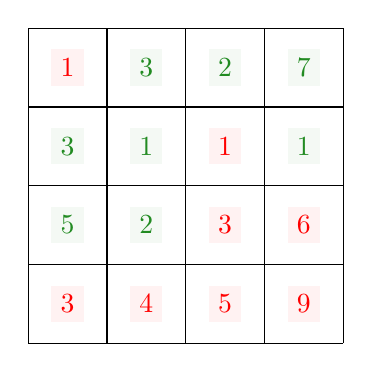
\begin{tikzpicture}
          \draw[step=1.0, black, thin, xshift=0.5cm, yshift=0.5cm] (0.0,0.0) grid (4.0,4.0);
          \draw (1.0, 4.0) node[Red, fill=Red!5] {$1$};
          \draw (2.0, 4.0) node[ForestGreen, fill=ForestGreen!5] {$3$};
          \draw (3.0, 4.0) node[ForestGreen, fill=ForestGreen!5] {$2$};
          \draw (4.0, 4.0) node[ForestGreen, fill=ForestGreen!5] {$7$};
          \draw (1.0, 3.0) node[ForestGreen, fill=ForestGreen!5] {$3$};
          \draw (2.0, 3.0) node[ForestGreen, fill=ForestGreen!5] {$1$};
          \draw (3.0, 3.0) node[Red, fill=Red!5] {$1$};
          \draw (4.0, 3.0) node[ForestGreen, fill=ForestGreen!5] {$1$};
          \draw (1.0, 2.0) node[ForestGreen, fill=ForestGreen!5] {$5$};
          \draw (2.0, 2.0) node[ForestGreen, fill=ForestGreen!5] {$2$};
          \draw (3.0, 2.0) node[Red, fill=Red!5] {$3$};
          \draw (4.0, 2.0) node[Red, fill=Red!5] {$6$};
          \draw (1.0, 1.0) node[Red, fill=Red!5] {$3$};
          \draw (2.0, 1.0) node[Red, fill=Red!5] {$4$};
          \draw (3.0, 1.0) node[Red, fill=Red!5] {$5$};
          \draw (4.0, 1.0) node[Red, fill=Red!5] {$9$};
        \end{tikzpicture}
        \caption{\centering State of the game. Player 1 has their meeple colored in $red$ and player 2 has theirs in $green$. We model player 1 defense strategy.}
        \label{fig:cos}
      \end{subfigure}
      \qquad
      \begin{subfigure}[b]{0.40\linewidth}
        \centering
        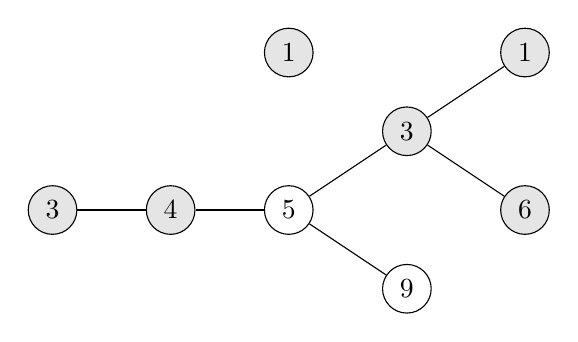
\begin{tikzpicture}
          \begin{scope}[every node/.style={circle,draw}]
            \node[color=Black,fill=Gray!20] (A) at (0.0,2.0) {3};
            \node[color=Black,fill=Gray!20] (B) at (1.5,2.0) {4};
            \node (C) at (3.0,2.0) {5};
            \node (D) at (4.5,1.0) {9};
            \node[color=Black,fill=Gray!20] (E) at (4.5,3.0) {3};
            \node[color=Black,fill=Gray!20] (F) at (6.0,4.0) {1};
            \node[color=Black,fill=Gray!20] (G) at (6.0,2.0) {6};
            \node[color=Black,fill=Gray!20] (H) at (3.0,4.0) {1};
          \end{scope}
          \begin{scope}[every node/.style={fill=white,circle}, every edge/.style={draw=black}]
            \draw [-] (A) edge (B);
            \draw [-] (B) edge (C);
            \draw [-] (C) edge (D);
            \draw [-] (C) edge (E);
            \draw [-] (E) edge (F);
            \draw [-] (E) edge (G);
          \end{scope}
        \end{tikzpicture}
        \caption{\centering A graph $G$ capturing the state of the board for player 1. As can be inferred from the graph, vulnerable regions are colored in $gray$.}
        \label{fig:sin}
      \end{subfigure}

      \caption{Graph construction/transformation.}
      \label{fig:plot}
    \end{figure}

    After the construction of $G$, we query and extract the disconnected subgraphs of $G$ containing
    at least one vertex colored in $gray$. These are precisely the connected regions of $G$ we want
    to fortify its borders against invading neighbors. To perform this fortification, we use the
    \textsc{Max-Flow} algorithm to dictate how many meeple pieces to move from one region to another
    and fortify regions of most need. Here conservation constraints will guaranteed that no meeple gets
    stuck in intermediate regions of the board during a migration. We discuss the details of the algorithm
    below which boils down to solving the circulation with demands problem.

    Firstly, we imagine the vertices of $G$ having supplies and demands. That is, if a vertex has supply
    of 2 then it can spare 2 more meeples than it receives. By symmetry, if a vertex has demand of 2 then
    it wants to receive 2 more meeples than it sends to its neighbors. We assing each vertex $v$ a value
    $\sigma_v$ that represents the ``excess'' at $v$---i.e., the difference between incoming meeples and
    outgoing ones. Note that $\sigma_v$ represents demand and when $\sigma_v < 0$ it represents supply.
    Then, the flow of conservation constraint could be replaced by the requirement that for each vertex
    $v$:
    \[
      \sum_{e=(*,v)} f_e - \sum_{e=(v,*)} f_e = \sigma_v
    \]
    We model this as a classical maximum flow problem by adding a source $s$ and a sink $t$. Whenever,
    a vertex $v$ has $\sigma_v > 0$, we add a directed edge $(v \rightarrow t)$ with capacity $\sigma_v$
    in the network flow. Likewise, whenever a vertex $v$ has $\sigma_v < 0$, we add and edge $(s \rightarrow
    v)$ with capacity $-\sigma_v$. We want to saturate all the edges going to $t$ to check if there is
    a way to satisfy all the demands in the network. If such demand is satisfied, then the maximum flow
    problem gives us the desired ``excess'' in each vertex, and consequently makes the weakest vulnarable
    region as strong as possible via the aforementioned demand and supply model.

    \vspace*{\baselineskip}
    {\itshape Time Analysis} \par
    Let $m$ be the number of rows in the board and $n$ the number of columns. Below is an itemized list of
    operations and costs incurred by the aforementioned algorithm:
    \begin{enumerate}[label={\arabic*.},itemsep=0mm]
      \item Constructing $G$ takes $O(mn)$.
      \item Extracting the connected components of $G$ takes $O(V+E)$.
      \item Filtering connected components that contain at least one vulnerable vertex takes $O(V)$.
      \item Running \textsc{Max-Flow} and assigning integral capacities takes at most $O(VE^2)$ via Edmonds-Karp.
    \end{enumerate}
    Hence the total running time of $O(VE^2)$.
\end{enumerate}
\end{document}
